\documentclass[11pt,a4paper]{article}
\usepackage[margin=1in]{geometry}
\usepackage{amsmath,amssymb}
\usepackage{hyperref}
\usepackage{graphicx}
\usepackage{algorithm}
\usepackage{algpseudocode}
\usepackage{siunitx}
\usepackage{ctex}

\title{数值偏微分方程课程报告1}
\author{陈柏锦}
\date{2025-10-13}

\begin{document}
\maketitle

\begin{abstract}
本文实现并应用CSR(Compressed Sparse Row,压缩行存储)格式来存储和计算由二维Dirichlet边界泊松方程离散产生的稀疏线性方程组。报告给出CSR核心要素、矩阵装配(包括普通矩形域与切除三角形形成的非凸域),以及基本运算(SpMV、上/下三角与对角提取)以支持Jacobi与Gauss--Seidel迭代。针对网格上标记为pt\_type=2的“近斜界面”点,本文根据实际代码(mesh.cpp)采用特殊非对称格式近似拉普拉斯,从而在靠近斜率为2的边界处获得更好的离散与求解性能。
\end{abstract}

\section{任务与目标}
实现CSR稀疏矩阵存储格式,核心功能:
\begin{enumerate}
  \item 存储元素:非零元个数 $nnz$、矩阵规模 $(m,n)$、每行起始位置(row\_ptr)、非零元列索引(col\_idx)以及元素值(val)。
  \item 构造稀疏矩阵:以二维Dirichlet边界泊松方程系数矩阵为例(五点格式为主),并支持通过屏蔽三角区域形成的非凸域。
  \item 基本操作:矩阵向量乘法(SpMV)、提取上下三角、提取对角线(服务于Jacobi/GS等迭代求解)。
\end{enumerate}

\section{CSR 存储格式}
CSR(行压缩)用三条数组表示 $A\in\mathbb{R}^{m\times n}$ 的非零结构:
\begin{itemize}
  \item \textbf{row\_ptr}(长度 $m+1$):第 $i$ 行的非零条目在 \texttt{col\_idx}/\texttt{val} 中的范围为 $[\texttt{row\_ptr}[i],\,\texttt{row\_ptr}[i{+}1])$。
  \item \textbf{col\_idx}(长度 $nnz$):对应非零条目的列索引(0-based)。
  \item \textbf{val}(长度 $nnz$):对应非零条目的数值。
\end{itemize}
元信息包括 $m,n,nnz$。装配时常由三元组$(i,j,\text{val})$累积后经排序与扫描压缩为CSR。

\section{二维泊松方程与矩阵装配}
考虑正拉普拉斯问题
\[
  \Delta u = f \quad \text{in } \Omega,\qquad
  u = g \quad \text{on } \partial\Omega,
\]
在规则张量网格上,内点 $(i,j)$ 的五点格式
\[
  \frac{u_{i-1,j}-2u_{i,j}+u_{i+1,j}}{h_x^2}
+ \frac{u_{i,j-1}-2u_{i,j}+u_{i,j+1}}{h_y^2} = f_{i,j}
\]
对应行系数:
\[
A_{p,p}=\frac{2}{h_x^2}+\frac{2}{h_y^2},\quad
A_{p,p\pm 1(\text{x邻})}=-\frac{1}{h_x^2},\quad
A_{p,p\pm n_x(\text{y邻})}=-\frac{1}{h_y^2}.
\]
Dirichlet 边界行替换为单位行:$A_{p,p}=1,\ b_p=g$。

\subsection{点类型与装配规则}
网格点按 \texttt{pt\_type} 分类:
\begin{itemize}
  \item \textbf{pt\_type=0(不可用)}:位于被切除三角形内部,不参与装配。
  \item \textbf{pt\_type=1(边界)}:Dirichlet 边界,行置单位,$b$ 取边值。
  \item \textbf{pt\_type=3(内部/常规)}:采用标准五点格式,持有左右上下四个邻接条目与对角线。
  \item \textbf{pt\_type=2(近斜界面)}:靠近斜率为2的斜界面(由三角切除形成的非凸边界)。为避免使用被移除点并增强稳定性,采用\emph{特殊非对称格式}近似 $\Delta u$(见下文)。
\end{itemize}

\subsection{近斜界面特殊格式(pt\_type=2)}
根据源码(mesh.cpp)对 \texttt{pt\_type=2} 的行,使用如下条目(只在相应邻居存在且为活动点时加入)。设当前活动点线性索引为 $p$,其四个特别使用的邻居为
$(i{-}1,j)$、$(i{+}1,j{+}1)$、$(i,j{-}1)$、$(i{-}1,j{-}1)$,则离散行中非对角与对角系数为
\[\begin{aligned}
A_{p,\,p(i-1,j)}   &= -\frac{2}{h_x^2},\\
A_{p,\,p(i,\,j-1)} &= -\frac{2}{h_y^2},\\
A_{p,\,p(i+1,j+1)} &= -\frac{1}{h_x h_y},\\
A_{p,\,p(i-1,j-1)} &= \phantom{-}\frac{1}{h_x h_y},\\
A_{p,p} &=-\!\!\!\sum_{\substack{q\neq p\\\text{同一行}}} A_{p,q}.
\end{aligned}\]
上述格式可理解为沿斜界面方向的一侧差分与混合项的组合,避免访问被移除区域的节点,同时在几何非凸、网格与界面不对齐的情形下,保持离散在预解后的对角占优性

\paragraph{说明} 对于 \texttt{pt\_type=2} 的条目,系数并非标准五点格式,包含了跨对角($(i\pm1,j\pm1)$)的混合项。实际装配时,仅当对应邻居有效(映射线性索引$\neq -1$)时才写入该非零元。

\section{CSR 基本操作}
\subsection{SpMV:$y \leftarrow Ax$}
CSR 的 SpMV 为逐行线性扫描(时间复杂度 $O(\text{nnz})$),访存连续,有利于缓存与向量化。

\subsection{提取上/下三角与对角线}
按行扫描,保留满足条件的条目并重建CSR:
\begin{itemize}
  \item 下三角 $R$(含对角):$j\le i$;
  \item 上三角 $U$(含对角):$j\ge i$;
  \item 对角线 $D$:$j=i$;若缺失可置 $\varepsilon$(提高迭代稳健性)。
\end{itemize}

\section{迭代方法与实现要点}
\paragraph{Jacobi}
$D=\text{diag}(A)$,$R=A-D$,更新
\[
x^{(k+1)} = D^{-1}(b - R\,x^{(k)}).
\]
实现上用一次非零线性扫描累加每行的非对角贡献(支持OpenMP并行),再并行更新新解。

\paragraph{Gauss--Seidel}
按行顺序前代入:
\[
x_i^{(k+1)}=\frac{1}{a_{ii}}\!\left(b_i-\sum_{j<i}a_{ij}x_j^{(k+1)}-\sum_{j>i}a_{ij}x_j^{(k)}\right).
\]
本工程采用对非零元单次线性扫描(先按行、列排序或直接利用CSR行段),在同一sweep中就地更新 $x$,避免重复索引与额外存储。

\section{数值实验与误差分析}
\paragraph{非凸域(切三角)}
通过屏蔽三组三角区域,形成不规则边界,靠近斜界面处采用 \texttt{pt\_type=2} 特殊格式。实验(日志)显示:$n=22817$(自由度),非零元$nnz=111{,}781$,GS 收敛迭代步数 $31194$,最终残差范数 $8.19\times 10^{-7}$,用时约 $15.41$s;误差指标 $\|e\|_\infty \approx 2.64\times 10^{-5}$,$\|e\|_{2} \approx 8.99\times 10^{-6}$。与标准五点相比,近界面处的非对称项能减少访问无效节点带来的误差与发散风险。

\paragraph{矩形域(naive)结果补充}
完整矩形域(无切除),外边界为Dirichlet 并使用同一解析解。该例装配得到 $nnz=162{,}693$,自由度 $n=33{,}153$。Gauss--Seidel 在容差 $10^{-10}$ 下收敛于第 $52055$ 次迭代;误差为
$\|e\|_\infty \approx 5.0\times 10^{-5}$,$\|e\|_{2} \approx 1.509\times 10^{-5}$。
在当前分辨率下,矩形域误差略高于非凸域结果,主要由于:
(i) 自由度增加使条件数增大,GS 收敛更慢,迭代终止时误差更受迭代误差影响;
(ii) 误差度量覆盖区域不同(非凸域排除了三角切除区),导致整体指标可有细微差异。
提升精度的途径包括网格加密、切换到更高效的Krylov方法(如CG/PCG)或多重网格预条件。

\begin{table}[h]
\centering
\begin{tabular}{lcccc}
\hline
案例 & 自由度 $n$ & 非零元 $nnz$ & GS迭代步 & 误差($\|e\|_\infty$ / $\|e\|_2$) \\
\hline
非凸域(R形) & 22{,}817 & 111{,}781 & 31{,}194 & $2.64\!\times\!10^{-5}$ / $8.99\!\times\!10^{-6}$ \\
矩形域 & 33{,}153 & 162{,}693 & 52{,}055 & $5.00\!\times\!10^{-5}$ / $1.509\!\times\!10^{-5}$ \\
\hline
\end{tabular}
\caption{两种区域下的装配规模、GS收敛与误差对比(公用解析解与边界条件)。}
\end{table}

\begin{figure}[h]
  \centering
  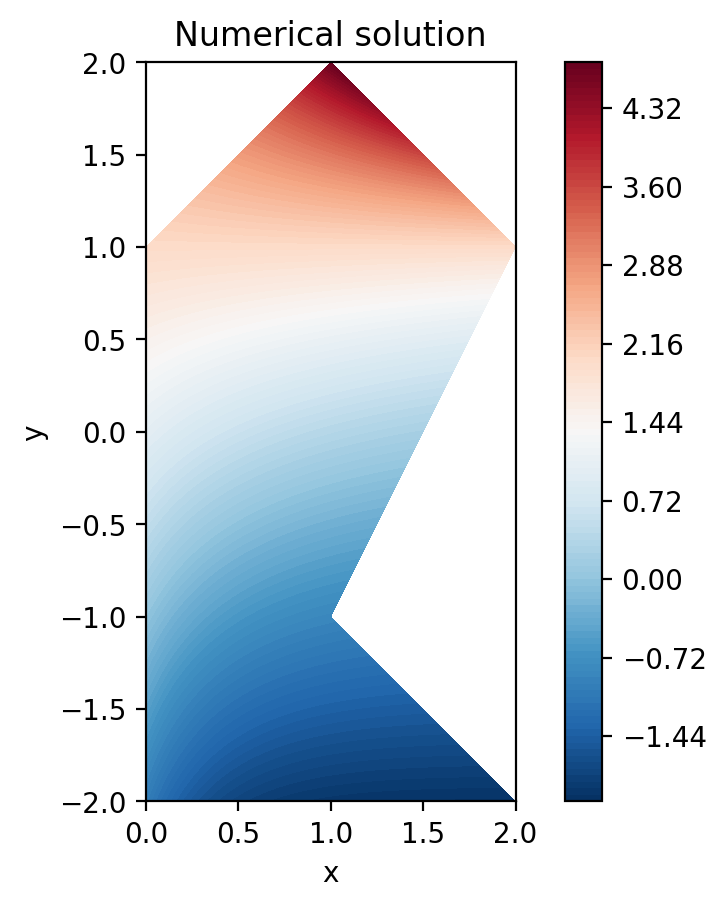
\includegraphics[width=0.46\linewidth]{../results/solution.png}\quad
  \includegraphics[width=0.46\linewidth]{../results/naive_rhs.png}
  \caption{左:非凸域数值解;右:矩形域数值解。}
\end{figure}

\section{结论}
本文实现了CSR稀疏格式、二维泊松方程系数矩阵装配与基本稀疏运算,并在Jacobi与Gauss--Seidel迭代中验证了其有效性。针对靠近斜率为2的复杂边界,代码对 \texttt{pt\_type=2} 采用了特殊非对称格式,既避免了访问被切除区域,又在数值上保持了良好收敛。

\paragraph{代码与数据}
矩阵与解存储于 \texttt{results/} 目录;绘图脚本见 \texttt{plot.py} 与 \texttt{naive.py}。

\end{document}